The following sections will give a short introduction of every main tool presented as relevant during the interviews and the additional research. 

\section{Alloy 4}


	\textbf{Developer}

	Company: 

	Webside:

	Contact address:

	Other  Participators:



	\textbf{Typical applications}

	Field of usage:

	%Brief introduction to what the tool does

	%Applicability
	%Key capabilities
	Input:

	Output:

	% Main restrictions e.g. only a subset of the target language is covered

	% Manual or automated use of the tool e.g. which steps are manual and automatic in the use of the tool.

	% Expertise level e.g. which prerequisite is needed to use the tool


	Integration in a tool chain
	%Currently distributed: Yes/No
	%Underlying technologies E.g. Framework, .NET vs. Java, etc.

	%Describe equirement to install/run the tool (all that is necessary to make the tool work fine: OS, Java version, dependencies with other tools, Eclipse version, ...)


	\textbf{License}


	\textbf{References}

	Bibliography:





\section{Artisan Studio}

	\textbf{Developer}

	Company: 

	Webside:

	Contact address:

	Other  Participators:



	\textbf{Typical applications}

	Field of usage:

	%Brief introduction to what the tool does

	%Applicability
	%Key capabilities
	Input:

	Output:

	% Main restrictions e.g. only a subset of the target language is covered

	% Manual or automated use of the tool e.g. which steps are manual and automatic in the use of the tool.

	% Expertise level e.g. which prerequisite is needed to use the tool


	Integration in a tool chain
	%Currently distributed: Yes/No
	%Underlying technologies E.g. Framework, .NET vs. Java, etc.

	%Describe equirement to install/run the tool (all that is necessary to make the tool work fine: OS, Java version, dependencies with other tools, Eclipse version, ...)


	\textbf{License}


	\textbf{References}

	Bibliography:


\section{Atelier B}

	\textbf{Developer}

	Company: 

	Webside:

	Contact address:

	Other  Participators:



	\textbf{Typical applications}

	Field of usage:

	%Brief introduction to what the tool does

	%Applicability
	%Key capabilities
	Input:

	Output:

	% Main restrictions e.g. only a subset of the target language is covered

	% Manual or automated use of the tool e.g. which steps are manual and automatic in the use of the tool.

	% Expertise level e.g. which prerequisite is needed to use the tool


	Integration in a tool chain
	%Currently distributed: Yes/No
	%Underlying technologies E.g. Framework, .NET vs. Java, etc.

	%Describe equirement to install/run the tool (all that is necessary to make the tool work fine: OS, Java version, dependencies with other tools, Eclipse version, ...)


	\textbf{License}


	\textbf{References}

	Bibliography:


\section{CompoSys}

	\textbf{Developer}

	Company: 

	Webside:

	Contact address:

	Other  Participators:



	\textbf{Typical applications}

	Field of usage:

	%Brief introduction to what the tool does

	%Applicability
	%Key capabilities
	Input:

	Output:

	% Main restrictions e.g. only a subset of the target language is covered

	% Manual or automated use of the tool e.g. which steps are manual and automatic in the use of the tool.

	% Expertise level e.g. which prerequisite is needed to use the tool


	Integration in a tool chain
	%Currently distributed: Yes/No
	%Underlying technologies E.g. Framework, .NET vs. Java, etc.

	%Describe equirement to install/run the tool (all that is necessary to make the tool work fine: OS, Java version, dependencies with other tools, Eclipse version, ...)


	\textbf{License}


	\textbf{References}

	Bibliography:


\section{Control Build}

	\textbf{Developer}

	Company: 

	Webside:

	Contact address:

	Other  Participators:



	\textbf{Typical applications}

	Field of usage:

	%Brief introduction to what the tool does

	%Applicability
	%Key capabilities
	Input:

	Output:

	% Main restrictions e.g. only a subset of the target language is covered

	% Manual or automated use of the tool e.g. which steps are manual and automatic in the use of the tool.

	% Expertise level e.g. which prerequisite is needed to use the tool


	Integration in a tool chain
	%Currently distributed: Yes/No
	%Underlying technologies E.g. Framework, .NET vs. Java, etc.

	%Describe equirement to install/run the tool (all that is necessary to make the tool work fine: OS, Java version, dependencies with other tools, Eclipse version, ...)


	\textbf{License}


	\textbf{References}

	Bibliography:


\section{CPN}

	\textbf{Developer}

	Company: 

	Webside:

	Contact address:

	Other  Participators:



	\textbf{Typical applications}

	Field of usage:

	%Brief introduction to what the tool does

	%Applicability
	%Key capabilities
	Input:

	Output:

	% Main restrictions e.g. only a subset of the target language is covered

	% Manual or automated use of the tool e.g. which steps are manual and automatic in the use of the tool.

	% Expertise level e.g. which prerequisite is needed to use the tool


	Integration in a tool chain
	%Currently distributed: Yes/No
	%Underlying technologies E.g. Framework, .NET vs. Java, etc.

	%Describe equirement to install/run the tool (all that is necessary to make the tool work fine: OS, Java version, dependencies with other tools, Eclipse version, ...)


	\textbf{License}


	\textbf{References}

	Bibliography:


\section{Enterprise Architect}

	\textbf{Developer}

	Company: 

	Webside:

	Contact address:

	Other  Participators:



	\textbf{Typical applications}

	Field of usage:

	%Brief introduction to what the tool does

	%Applicability
	%Key capabilities
	Input:

	Output:

	% Main restrictions e.g. only a subset of the target language is covered

	% Manual or automated use of the tool e.g. which steps are manual and automatic in the use of the tool.

	% Expertise level e.g. which prerequisite is needed to use the tool


	Integration in a tool chain
	%Currently distributed: Yes/No
	%Underlying technologies E.g. Framework, .NET vs. Java, etc.

	%Describe equirement to install/run the tool (all that is necessary to make the tool work fine: OS, Java version, dependencies with other tools, Eclipse version, ...)


	\textbf{License}


	\textbf{References}

	Bibliography:


\section{ERTMS FormalSpecs}

	\textbf{Developer}

	Company: 

	Webside:

	Contact address:

	Other  Participators:



	\textbf{Typical applications}

	Field of usage:

	%Brief introduction to what the tool does

	%Applicability
	%Key capabilities
	Input:

	Output:

	% Main restrictions e.g. only a subset of the target language is covered

	% Manual or automated use of the tool e.g. which steps are manual and automatic in the use of the tool.

	% Expertise level e.g. which prerequisite is needed to use the tool


	Integration in a tool chain
	%Currently distributed: Yes/No
	%Underlying technologies E.g. Framework, .NET vs. Java, etc.

	%Describe equirement to install/run the tool (all that is necessary to make the tool work fine: OS, Java version, dependencies with other tools, Eclipse version, ...)


	\textbf{License}


	\textbf{References}

	Bibliography:


\section{Frama-C}

	\textbf{Developer}

	Company: 

	Webside:

	Contact address:

	Other  Participators:



	\textbf{Typical applications}

	Field of usage:

	%Brief introduction to what the tool does

	%Applicability
	%Key capabilities
	Input:

	Output:

	% Main restrictions e.g. only a subset of the target language is covered

	% Manual or automated use of the tool e.g. which steps are manual and automatic in the use of the tool.

	% Expertise level e.g. which prerequisite is needed to use the tool


	Integration in a tool chain
	%Currently distributed: Yes/No
	%Underlying technologies E.g. Framework, .NET vs. Java, etc.

	%Describe equirement to install/run the tool (all that is necessary to make the tool work fine: OS, Java version, dependencies with other tools, Eclipse version, ...)


	\textbf{License}


	\textbf{References}

	Bibliography:


\section{iglos}

	\textbf{Developer}

	Company: 

	Webside:

	Contact address:

	Other  Participators:



	\textbf{Typical applications}

	Field of usage:

	%Brief introduction to what the tool does

	%Applicability
	%Key capabilities
	Input:

	Output:

	% Main restrictions e.g. only a subset of the target language is covered

	% Manual or automated use of the tool e.g. which steps are manual and automatic in the use of the tool.

	% Expertise level e.g. which prerequisite is needed to use the tool


	Integration in a tool chain
	%Currently distributed: Yes/No
	%Underlying technologies E.g. Framework, .NET vs. Java, etc.

	%Describe equirement to install/run the tool (all that is necessary to make the tool work fine: OS, Java version, dependencies with other tools, Eclipse version, ...)


	\textbf{License}


	\textbf{References}

	Bibliography:


\section{iLock/iCertifier}

	\textbf{Developer}

	Company: 

	Webside:

	Contact address:

	Other  Participators:



	\textbf{Typical applications}

	Field of usage:

	%Brief introduction to what the tool does

	%Applicability
	%Key capabilities
	Input:

	Output:

	% Main restrictions e.g. only a subset of the target language is covered

	% Manual or automated use of the tool e.g. which steps are manual and automatic in the use of the tool.

	% Expertise level e.g. which prerequisite is needed to use the tool


	Integration in a tool chain
	%Currently distributed: Yes/No
	%Underlying technologies E.g. Framework, .NET vs. Java, etc.

	%Describe equirement to install/run the tool (all that is necessary to make the tool work fine: OS, Java version, dependencies with other tools, Eclipse version, ...)


	\textbf{License}


	\textbf{References}

	Bibliography:


\section{KNOW Enterprise}

	\textbf{Developer}

	Company: 

	Webside:

	Contact address:

	Other  Participators:



	\textbf{Typical applications}

	Field of usage:

	%Brief introduction to what the tool does

	%Applicability
	%Key capabilities
	Input:

	Output:

	% Main restrictions e.g. only a subset of the target language is covered

	% Manual or automated use of the tool e.g. which steps are manual and automatic in the use of the tool.

	% Expertise level e.g. which prerequisite is needed to use the tool


	Integration in a tool chain
	%Currently distributed: Yes/No
	%Underlying technologies E.g. Framework, .NET vs. Java, etc.

	%Describe equirement to install/run the tool (all that is necessary to make the tool work fine: OS, Java version, dependencies with other tools, Eclipse version, ...)


	\textbf{License}


	\textbf{References}

	Bibliography:


\section{MagicDraw}

	\textbf{Developer}

	Company: 

	Webside:

	Contact address:

	Other  Participators:



	\textbf{Typical applications}

	Field of usage:

	%Brief introduction to what the tool does

	%Applicability
	%Key capabilities
	Input:

	Output:

	% Main restrictions e.g. only a subset of the target language is covered

	% Manual or automated use of the tool e.g. which steps are manual and automatic in the use of the tool.

	% Expertise level e.g. which prerequisite is needed to use the tool


	Integration in a tool chain
	%Currently distributed: Yes/No
	%Underlying technologies E.g. Framework, .NET vs. Java, etc.

	%Describe equirement to install/run the tool (all that is necessary to make the tool work fine: OS, Java version, dependencies with other tools, Eclipse version, ...)


	\textbf{License}


	\textbf{References}

	Bibliography:


\section{mCRL2}

	\textbf{Developer}

	Company: 

	Webside:

	Contact address:

	Other  Participators:



	\textbf{Typical applications}

	Field of usage:

	%Brief introduction to what the tool does

	%Applicability
	%Key capabilities
	Input:

	Output:

	% Main restrictions e.g. only a subset of the target language is covered

	% Manual or automated use of the tool e.g. which steps are manual and automatic in the use of the tool.

	% Expertise level e.g. which prerequisite is needed to use the tool


	Integration in a tool chain
	%Currently distributed: Yes/No
	%Underlying technologies E.g. Framework, .NET vs. Java, etc.

	%Describe equirement to install/run the tool (all that is necessary to make the tool work fine: OS, Java version, dependencies with other tools, Eclipse version, ...)


	\textbf{License}


	\textbf{References}

	Bibliography:


\section{Modelio}

	\textbf{Developer}

	Company: 

	Webside:

	Contact address:

	Other  Participators:



	\textbf{Typical applications}

	Field of usage:

	%Brief introduction to what the tool does

	%Applicability
	%Key capabilities
	Input:

	Output:

	% Main restrictions e.g. only a subset of the target language is covered

	% Manual or automated use of the tool e.g. which steps are manual and automatic in the use of the tool.

	% Expertise level e.g. which prerequisite is needed to use the tool


	Integration in a tool chain
	%Currently distributed: Yes/No
	%Underlying technologies E.g. Framework, .NET vs. Java, etc.

	%Describe equirement to install/run the tool (all that is necessary to make the tool work fine: OS, Java version, dependencies with other tools, Eclipse version, ...)


	\textbf{License}


	\textbf{References}

	Bibliography:


\section{NuSMV}

	\textbf{Developer}

	Company: 

	Webside:

	Contact address:

	Other  Participators:



	\textbf{Typical applications}

	Field of usage:

	%Brief introduction to what the tool does

	%Applicability
	%Key capabilities
	Input:

	Output:

	% Main restrictions e.g. only a subset of the target language is covered

	% Manual or automated use of the tool e.g. which steps are manual and automatic in the use of the tool.

	% Expertise level e.g. which prerequisite is needed to use the tool


	Integration in a tool chain
	%Currently distributed: Yes/No
	%Underlying technologies E.g. Framework, .NET vs. Java, etc.

	%Describe equirement to install/run the tool (all that is necessary to make the tool work fine: OS, Java version, dependencies with other tools, Eclipse version, ...)


	\textbf{License}


	\textbf{References}

	Bibliography:


\section{Papyrus}

	\textbf{Developer}

	Company: 

	Webside:

	Contact address:

	Other  Participators:



	\textbf{Typical applications}

	Field of usage:

	%Brief introduction to what the tool does

	%Applicability
	%Key capabilities
	Input:

	Output:

	% Main restrictions e.g. only a subset of the target language is covered

	% Manual or automated use of the tool e.g. which steps are manual and automatic in the use of the tool.

	% Expertise level e.g. which prerequisite is needed to use the tool


	Integration in a tool chain
	%Currently distributed: Yes/No
	%Underlying technologies E.g. Framework, .NET vs. Java, etc.

	%Describe equirement to install/run the tool (all that is necessary to make the tool work fine: OS, Java version, dependencies with other tools, Eclipse version, ...)


	\textbf{License}


	\textbf{References}

	Bibliography:


\section{Perfect Developer}

	\textbf{Developer}

	Company: 

	Webside:

	Contact address:

	Other  Participators:



	\textbf{Typical applications}

	Field of usage:

	%Brief introduction to what the tool does

	%Applicability
	%Key capabilities
	Input:

	Output:

	% Main restrictions e.g. only a subset of the target language is covered

	% Manual or automated use of the tool e.g. which steps are manual and automatic in the use of the tool.

	% Expertise level e.g. which prerequisite is needed to use the tool


	Integration in a tool chain
	%Currently distributed: Yes/No
	%Underlying technologies E.g. Framework, .NET vs. Java, etc.

	%Describe equirement to install/run the tool (all that is necessary to make the tool work fine: OS, Java version, dependencies with other tools, Eclipse version, ...)


	\textbf{License}


	\textbf{References}

	Bibliography:


\section{PRISM}
	\textbf{Developer}

	Company: 

	Webside:

	Contact address:

	Other  Participators:



	\textbf{Typical applications}

	Field of usage:

	%Brief introduction to what the tool does

	%Applicability
	%Key capabilities
	Input:

	Output:

	% Main restrictions e.g. only a subset of the target language is covered

	% Manual or automated use of the tool e.g. which steps are manual and automatic in the use of the tool.

	% Expertise level e.g. which prerequisite is needed to use the tool


	Integration in a tool chain
	%Currently distributed: Yes/No
	%Underlying technologies E.g. Framework, .NET vs. Java, etc.

	%Describe equirement to install/run the tool (all that is necessary to make the tool work fine: OS, Java version, dependencies with other tools, Eclipse version, ...)


	\textbf{License}


	\textbf{References}

	Bibliography:


\section{ProB}

	\textbf{Developer}

	Company: 

	Webside:

	Contact address:

	Other  Participators:



	\textbf{Typical applications}

	Field of usage:

	%Brief introduction to what the tool does

	%Applicability
	%Key capabilities
	Input:

	Output:

	% Main restrictions e.g. only a subset of the target language is covered

	% Manual or automated use of the tool e.g. which steps are manual and automatic in the use of the tool.

	% Expertise level e.g. which prerequisite is needed to use the tool


	Integration in a tool chain
	%Currently distributed: Yes/No
	%Underlying technologies E.g. Framework, .NET vs. Java, etc.

	%Describe equirement to install/run the tool (all that is necessary to make the tool work fine: OS, Java version, dependencies with other tools, Eclipse version, ...)


	\textbf{License}


	\textbf{References}

	Bibliography:


\section{ProR}

	\textbf{Developer}

	Company: 

	Webside:

	Contact address:

	Other  Participators:



	\textbf{Typical applications}

	Field of usage:

	%Brief introduction to what the tool does

	%Applicability
	%Key capabilities
	Input:

	Output:

	% Main restrictions e.g. only a subset of the target language is covered

	% Manual or automated use of the tool e.g. which steps are manual and automatic in the use of the tool.

	% Expertise level e.g. which prerequisite is needed to use the tool


	Integration in a tool chain
	%Currently distributed: Yes/No
	%Underlying technologies E.g. Framework, .NET vs. Java, etc.

	%Describe equirement to install/run the tool (all that is necessary to make the tool work fine: OS, Java version, dependencies with other tools, Eclipse version, ...)


	\textbf{License}


	\textbf{References}

	Bibliography:


\section{Rational Architect}

	\textbf{Developer}

	Company: 

	Webside:

	Contact address:

	Other  Participators:



	\textbf{Typical applications}

	Field of usage:

	%Brief introduction to what the tool does

	%Applicability
	%Key capabilities
	Input:

	Output:

	% Main restrictions e.g. only a subset of the target language is covered

	% Manual or automated use of the tool e.g. which steps are manual and automatic in the use of the tool.

	% Expertise level e.g. which prerequisite is needed to use the tool


	Integration in a tool chain
	%Currently distributed: Yes/No
	%Underlying technologies E.g. Framework, .NET vs. Java, etc.

	%Describe equirement to install/run the tool (all that is necessary to make the tool work fine: OS, Java version, dependencies with other tools, Eclipse version, ...)


	\textbf{License}


	\textbf{References}

	Bibliography:


\section{SCADE Suite / SCADE System / SCADE LifeCycle}

	\textbf{Developer}

	Company: Esterel Technologies S.A.

	Webside: \url{http://esterel-technologies.com/} \\[2pt]

	Contact address: Parc Euclide, 8 rue Blaise Pasc, 78990 Elancourt, France

	Other  Participators:

	\textbf{Typical applications}

	Field of usage:
	Safety critical systems like
\vspace{-10pt}
\begin{itemize}[topsep=2pt, partopsep=2pt,itemsep=2pt,parsep=2pt]
  \item Rail interlocking systems
  \item Rail track vacancy detection systems
  \item Rail train control systems
  \item Rail Level-crossing protection systems
  \item Avionic flight controller
\end{itemize}

	%Brief introduction to what the tool does
\begin{figure}[h]
\centering
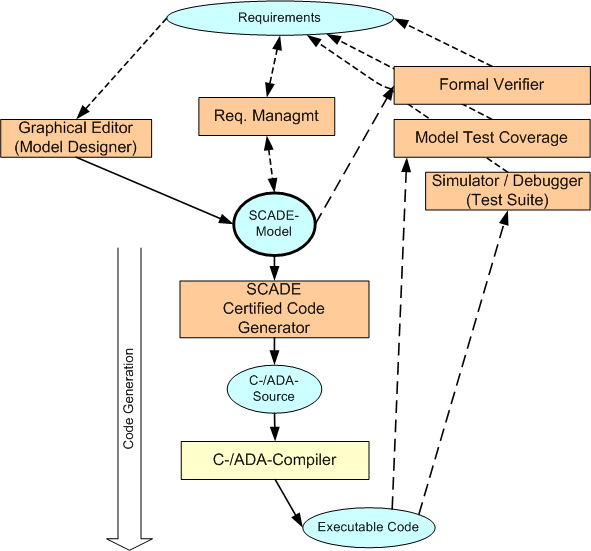
\includegraphics[scale=0.6]{SCADE_Overview.png}
\caption{SCADE Suite Overview}
\label{fig:SCADE_Suite_Overview}
\end{figure}

	%Applicability
	
SCADE is a formal modelling language targeted for safety-critical embedded control applications in the avionics, rail, automotive and industrial automation domain. SCADE source code can be written as text (for anyone who likes writing plain text) or (more usual) as schematic diagrams. SCADE models are synchronously clocked data flow and state machines, that can be nested and intermixed with each other without limitations. 
SCADE provides DO-178B- and EN50128-certified code generators producing C or ADA code as output. SCADE models are therefore concrete, deterministic, executable and verifiable; it allows the production of rapid prototype as well as of safety related target system software. 

SCADE comes with an integrated development environment (SCADE Suite IDE) including code generator, graphical simulator, model checker/prover, model test coverage analyzer, report generators, version and requirements management gateway with interfaces to various other tools like static code and timing analyzers, System/SysML modelling tools etc.. The IDE provides automatization interfaces to be controlled from external tools, and all SCADE tools itself can also be used in batch mode. In addition, plugins for Eclipse integration are available. 

The SCADE paradigm of synchronously clocked data flow and state machines works perfect for embedded control or industry automation software. It is less suitable for tasks like text processing or computer graphic applications. SCADE models do not only describe the structure of software; instead, they are the software implementation itself too. System architectures typically require a higher abstraction means of description at top level like SysML. While SysML modelling can be achieved with any SysML tools, SCADE System provides an automatic transformation from SysML to SCADE. 

For a start with SCADE a learning phase of one week should be planned.   

	\textbf{License}
	
	Commercial licenses + academic license program


	\textbf{References}

	Bibliography:
	
	\url{http://www.interested-ip.eu/}\\[4pt]
	\url{http://http://www.interested-ip.eu/final-report.html/} \\[4pt]


\section{Simulink/ Design Verifier}

	\textbf{Developer}

	Company: 

	Webside:

	Contact address:

	Other  Participators:



	\textbf{Typical applications}

	Field of usage:

	%Brief introduction to what the tool does

	%Applicability
	%Key capabilities
	Input:

	Output:

	% Main restrictions e.g. only a subset of the target language is covered

	% Manual or automated use of the tool e.g. which steps are manual and automatic in the use of the tool.

	% Expertise level e.g. which prerequisite is needed to use the tool


	Integration in a tool chain
	%Currently distributed: Yes/No
	%Underlying technologies E.g. Framework, .NET vs. Java, etc.

	%Describe equirement to install/run the tool (all that is necessary to make the tool work fine: OS, Java version, dependencies with other tools, Eclipse version, ...)


	\textbf{License}


	\textbf{References}

	Bibliography:


\section{SPARK GPL/ GNATprove}

	\textbf{Developer}

	Company: 

	Webside:

	Contact address:

	Other  Participators:



	\textbf{Typical applications}

	Field of usage:

	%Brief introduction to what the tool does

	%Applicability
	%Key capabilities
	Input:

	Output:

	% Main restrictions e.g. only a subset of the target language is covered

	% Manual or automated use of the tool e.g. which steps are manual and automatic in the use of the tool.

	% Expertise level e.g. which prerequisite is needed to use the tool


	Integration in a tool chain
	%Currently distributed: Yes/No
	%Underlying technologies E.g. Framework, .NET vs. Java, etc.

	%Describe equirement to install/run the tool (all that is necessary to make the tool work fine: OS, Java version, dependencies with other tools, Eclipse version, ...)


	\textbf{License}


	\textbf{References}

	Bibliography:


\section{SPIN}

	\textbf{Developer}

	Company: 

	Webside:

	Contact address:

	Other  Participators:



	\textbf{Typical applications}

	Field of usage:

	%Brief introduction to what the tool does

	%Applicability
	%Key capabilities
	Input:

	Output:

	% Main restrictions e.g. only a subset of the target language is covered

	% Manual or automated use of the tool e.g. which steps are manual and automatic in the use of the tool.

	% Expertise level e.g. which prerequisite is needed to use the tool


	Integration in a tool chain
	%Currently distributed: Yes/No
	%Underlying technologies E.g. Framework, .NET vs. Java, etc.

	%Describe equirement to install/run the tool (all that is necessary to make the tool work fine: OS, Java version, dependencies with other tools, Eclipse version, ...)


	\textbf{License}


	\textbf{References}

	Bibliography:


\section{$\pi$-Tool}

	\textbf{Developer}

	Company: 

	Webside:

	Contact address:

	Other  Participators:



	\textbf{Typical applications}

	Field of usage:

	%Brief introduction to what the tool does

	%Applicability
	%Key capabilities
	Input:

	Output:

	% Main restrictions e.g. only a subset of the target language is covered

	% Manual or automated use of the tool e.g. which steps are manual and automatic in the use of the tool.

	% Expertise level e.g. which prerequisite is needed to use the tool


	Integration in a tool chain
	%Currently distributed: Yes/No
	%Underlying technologies E.g. Framework, .NET vs. Java, etc.

	%Describe equirement to install/run the tool (all that is necessary to make the tool work fine: OS, Java version, dependencies with other tools, Eclipse version, ...)


	\textbf{License}


	\textbf{References}

	Bibliography: